\documentclass[a4paper,11pt]{beamer}
\usepackage[utf8]{inputenc}
\usepackage{lmodern}
\usepackage{caption}
\usepackage{subcaption}
% Thème Darmstadt
\usetheme{Darmstadt}
\usepackage{graphicx}
\usepackage{caption}
\usepackage{ragged2e}
\usepackage{listings}
\usepackage{color}
\usepackage{gitdags}
\usepackage{fontawesome, wasysym}
%\captionsetup[figure]{labelformat=empty}

\setbeamertemplate{navigation symbols}{} 
\setbeamertemplate{footline} 
{  
	\begin{beamercolorbox}[ht=2.5ex,dp=1.125ex,%
      leftskip=.3cm,rightskip=.3cm plus1fil]{title in head/foot}%
      {\usebeamerfont{title in head/foot}\insertshorttitle} \hfill    
      \insertframenumber / \inserttotalframenumber%
    \end{beamercolorbox}%
%     \begin{beamercolorbox}[colsep=1.5pt]{lower separation line foot}
%     \end{beamercolorbox} 
}

% Informations sur la présentation
\title{Gestion de code avec Git (FIEC30EM)}
\author{frank.buloup@univ-amu.fr} 
\institute{Aix Marseille Université\\Faculté des Sciences du Sport\\Master 2 IEAP - Facteurs Humains}
\date{}

\newcounter{exampleBlockCounter}
\setcounter{exampleBlockCounter}{1} 

\definecolor{comment}{rgb}{0.12, 0.38, 0.18 } %adjusted, in Eclipse: {0.25, 0.42, 0.30 } = #3F6A4D
\definecolor{keyword}{rgb}{0.37, 0.08, 0.25}  % #5F1441
\definecolor{string}{rgb}{0.06, 0.10, 0.98} % 

\lstset{
language=Python,
frame=single,
frameround=tttt,
rulesepcolor=\color{black},
showspaces=false,showtabs=false,tabsize=2,
numberstyle=\tiny,numbers=left,
stringstyle=\color{string},
keywordstyle = \color{keyword}\bfseries,
commentstyle=\color{comment}\itshape,
basicstyle=\ttfamily\footnotesize,
breaklines=true,
captionpos=b
}

%\includeonlyframes{current}

\begin{document}

% Première diapositive : Titre
\begin{frame}[plain]
    \titlepage
    \center{
\includegraphics[scale=0.75]{images/by-nc-sa.eps}}
 	\vspace{0.5cm}

	
\includegraphics[scale=0.6]{images/LogoAMU.png}\hspace*{2cm}
	
\includegraphics[scale=0.35]{images/LogoCNRS.eps}\hspace*{2cm}
	
\includegraphics[scale=0.09]{images/LogoISM.eps}
    
\end{frame}

\begin{frame}{Gestion de code avec Git}
	\tableofcontents[hideallsubsections]
\end{frame}

\AtBeginSection{%
    \begin{frame}
        \tableofcontents[sections=\value{section}]
    \end{frame}
}

\section{Introduction \& Installation de Git}
\subsection{Objectifs du module \& Organisation}
\begin{frame}

\center
À l'issue de cette formation, vous serez capable de :
\vspace{0.25cm}

\begin{enumerate}
\item Mettre en œuvre une petite plateforme d'acquisition de données
	\begin{enumerate}
		\item Utiliser Arduino IDE et un Uno R4 pour l'acquisition des données 
		\item Utiliser Python pour créer un gestionnaire d'essai
		\item Utiliser Python pour le traitement des données
	\end{enumerate}
\item Mettre en œuvre un projet en mode collaboratif avec Git sur GitHub
	\begin{enumerate}
		\item Décrire les principes de fonctionnement d'un gestionnaire de versions distribué
		\item Créer, initialiser et cloner un dépôt avec Git
		\item Manipuler les commandes de Git pour gérer les fichiers et les branches
		\item Résoudre les conflits de fusion
	\end{enumerate}
\end{enumerate}
\end{frame}

\begin{frame}
	\begin{block}{Organisation}
		\begin{itemize}
			\item Un projet par équipe pour mettre en œuvre ces apprentissages
			\item Cours et TDs pour apprendre les bases de Git			
			\item Deux (à trois) étudiants par équipe
		\end{itemize}
	\end{block}

	\begin{block}{Volumes horaires}
		\begin{itemize}
			\item Environ 14 heures pour le projet
			\item Environ 4 heures de cours/TDs
%			\item Environ 2 heures pour l'oral de présentation du projet
		\end{itemize}
	\end{block}
	\begin{alertblock}{Evaluation}
		\begin{itemize}
			\item 50\% sur un CC Git (examen écrit 30mn)
			\item 50\% sur le projet tout au long du module
			%\item 50\% sur une présentation orale du projet par équipe
			%	\begin{itemize}
			%		\item 10mn de présentation
			%		\item 5mn de questions
			%		\item Grille d'évaluation
			%	\end{itemize}
		\end{itemize}
	\end{alertblock}
\end{frame}

\subsection{les projets \& Les comptes GitHub}
\begin{frame}	
	\begin{block}{Les projets}
	Sur la base d'un Arduino Uno R4 Wifi avec :
		\begin{itemize}
			\item une jauge de contrainte (2 postes)
			\item une résistance à détection de force (2 postes)
			\item un capteur à ultrason (2 postes)
			\item \textcolor{red}{un potentiomètre}
			\item \textcolor{red}{un codeur optique}
		\end{itemize}
	\end{block}
	\begin{block}{Comptes GitHub}
		\begin{itemize}
			\item Création de comptes sur GitHub
			\item Compte du Master : MasterFHGit
		\end{itemize}	
	\end{block}	
\end{frame}

\subsection{Les projets : c'est parti dès maintenant !}
\begin{frame}

\begin{block}{Les projets - Répartition par binômes voire trinômes}
Sur la base d'un Arduino Uno R4 Wifi avec :
	\begin{itemize}
		\item une jauge de contrainte (2 postes - 2x2 étudiants)
		\item une résistance à détection de force (2 postes - 2x2 étudiants)
		\item un capteur à ultrason (2 postes - 2x2 étudiants)
		\item \textcolor{red}{un potentiomètre - 2 étudiants}
		\item \textcolor{red}{un codeur optique - 2 étudiants}
	\end{itemize}
\end{block}
\centering

\normalsize
\textcolor{blue}{\textbf{\underline{\href{https://raw.githubusercontent.com/fbuloup/CodeManagementWithGit/main/projets.pdf}{Veuillez suivre ce lien pour démarrer le projet dès maintenant}}}}	
\end{frame}

\subsection{Installation de git en local : commandes de base}
\begin{frame}
\begin{exampleblock}{Exercice \Roman{exampleBlockCounter} - Étapes 1 \& 2 du projet}\stepcounter{exampleBlockCounter} 
\begin{enumerate}
    \item Installer Git en suivant le lien suivant : \textcolor{blue}{\textbf{\underline{\href{https://git-scm.com}{Git - SCM}}}}
    \center{
        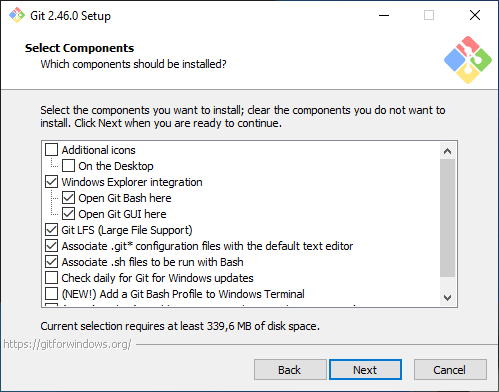
\includegraphics[scale=0.3]{images/GitInstaller.PNG}
        \captionof{figure}{Git Setup - Garder les options par défaut}}
\end{enumerate}

\begin{enumerate}
	\setcounter{enumi}{1}
    \item Initialiser votre dossier dans git : commande "git init"
    \item Ajouter les fichiers : commande "git add"
    \item Archiver cette première étape : commande "git commit"
    \item Continuer pour archiver l'étape 2 du projet 
\end{enumerate}

\end{exampleblock}
\end{frame}

\subsection{Concepts fondamentaux}
\begin{frame}
\begin{block}{État initial après le premier commit local}
\centering
\begin{tikzpicture}
	\gitDAG[grow right sep = 2em]{ad6c0bb};
    \gitremotebranch
    	[main]    % node name
    	{main} % node text
        {right=of ad6c0bb}    % node placement
        {ad6c0bb}             % target
     \gitHEAD
        {above=of main} % node placement
        {main}          % target
\end{tikzpicture}
\begin{itemize}
	\item \textbf{ad6c0bb} est l'ID du commit (l'ID complet est un SHA1)
	\item \textbf{main} est une référence au dernier commit de la branche qui porte le même nom
	\item On peut avoir plusieurs branches et donc plusieurs références (\textbf{main}, \textbf{dev}, \textbf{feature1} etc.)
\end{itemize}


\end{block}
\end{frame}

\begin{frame}
\begin{block}{État après le deuxième commit local}
\centering
\begin{tikzpicture}
	\gitDAG[grow right sep = 2em]{ad6c0bb -- 55e023d};
    \gitremotebranch
    	[main]    % node name
    	{main} % node text
        {right=of 55e023d}    % node placement
        {55e023d}             % target
     \gitHEAD
        {above=of main} % node placement
        {main}  
\end{tikzpicture}
\begin{itemize}
	\item \textbf{main} est par convention un nom de branche de production (branche principale)
	\item On peut aussi trouver \textbf{master} à la place de \textbf{main} mais de moins en moins
\end{itemize}
\end{block}
\end{frame}

\begin{frame}
\begin{alertblock}{Heads}
\justifying
A head is simply a reference to a commit object. Each head has a name. By default, there is a head in every repository called master (or main). A repository can contain any number of heads. At any given time, one head is selected as the “current head.” This head is aliased to HEAD, always in capitals.

Note this difference: a “head” (lowercase) refers to any one of the named heads in the repository; “HEAD” (uppercase) refers exclusively to the currently active head. This distinction is used frequently in Git documentation.
\end{alertblock}
\centering
\textcolor{blue}{
\textbf{\underline{\href{https://www.cduan.com/technical/git/git-1.shtml\#heads}{Git - Heads}}}}
\end{frame}

\subsection{Les zones de Git}
\begin{frame}[containsverbatim]
    \center{
        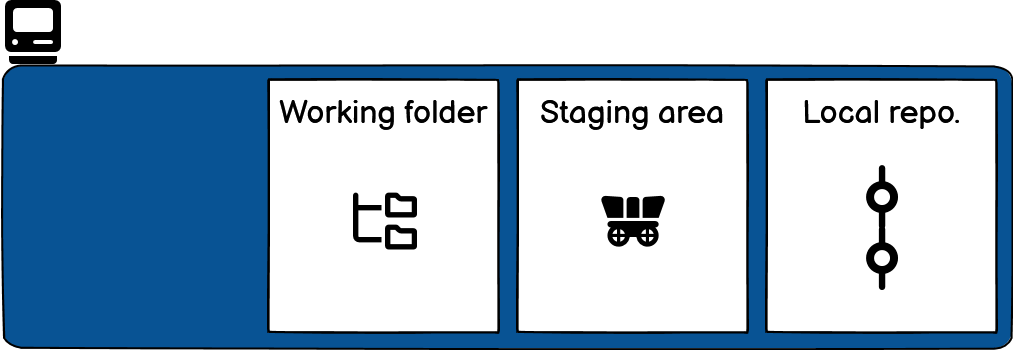
\includegraphics[scale=0.4]{images/zones1_local.png}}
\end{frame}


\section{Présentation \& Utilisation de Git}
\subsection{Git ? C'est quoi ?}
\begin{frame}

\begin{block}{Git ? C'est quoi ?}
\centering

\includegraphics[scale=0.1]{images/git.png} 
\end{block}
\centering
	\huge \textbf{Une idée ?}
	
\normalsize
\textcolor{blue}{\textbf{\underline{\href{https://git-scm.com}{Documentation Git}}}}	
	
\end{frame}

\begin{frame}
    \begin{block}{Git n'est pas un serveur (au sens centralisé)}
    \begin{itemize}
    \item Git n'offre pas de fonctionnalité de gestion de projet complète (e.g. gestion de tâches, de bugs ou wiki)
   \item Github et GitLab sont deux exemples de solutions complètes
     \end{itemize}
    \centering
        \begin{tabular}{c c c c}
            
\includegraphics[scale=0.1]{images/github.png} & 
\includegraphics[scale=0.066]{images/gitlab.png} & 
\includegraphics[scale=0.08]{images/bitbucket.png} & 
\includegraphics[scale=0.045]{images/gitea.png} \\
            \textbf{Github} & \textbf{GitLab}  & \textbf{Bitbucket} & \textbf{Gitea} 
        \end{tabular}
        
    \end{block}
    \pause
    \begin{block}{Git n'est pas un espace de stockage de fichiers type Dropbox}
        \begin{itemize}
            \item Pas de sauvegarde automatique des fichiers
            \item Pas de gestion optimale des fichiers volumineux$^*$ ou binaires$^{**}$
        \end{itemize}
    \end{block}
\vspace{.125cm}

\centering
\footnotesize $^{*}$Dans ce cas, on peut utiliser une extension spécifique : git LFS\\
\footnotesize $^{**}$Les fichiers binaires ne sont pas très lisibles (git diff !!!)
\end{frame}

\begin{frame}
    \begin{block}{Git est un système de contrôle de version (Version Control System)}
        \begin{itemize}
            \item Historique des versions de tous les fichiers
            \item Manipulation complète de l'historique possible
            \item Décentralisé (bientôt plus clair...)
            \item On trouve aussi : "Source Code Management System"
        \end{itemize}
    \end{block}
    \pause
    \begin{block}{Pourquoi gérer des versions de fichiers, utiliser un VCS ?}
        \begin{itemize}
            \item Pour pouvoir revenir en arrière
            \item Pour comparer des versions de fichiers
            \item Pour expérimenter, tester des idées
            \item Pour travailler à plusieurs plus facilement
        \end{itemize}
    \end{block}
    
\end{frame}

\begin{frame}
\centering {\huge \textbf{\textcolor{red}{Vous pouvez gérer tous types de fichiers avec git !}}}
\begin{block}{Exemples de fichiers gérés par git}
\begin{itemize}
\item Fichiers de code informatique
\item Fichiers textes (e.g. .doc)
\item Fichiers binaires (e.g. images, sons) - Si volumineux : git LFS$^{*}$
\item Fichiers de données - Si volumineux : git LFS$^{*}$
\item Documentation de projets (cahier des charges, devis...)
\item etc.
\end{itemize}
\end{block}
\vspace{.25cm}

\centering {\huge \textbf{\textcolor{red}{Gestion collaborative de projets}}}
\vspace{.25cm}

\footnotesize $^{*}$Utilisation de l'extension \textcolor{blue}{\textbf{\underline{\href{https://git-lfs.com/}{Git Large File Storage}}}}\\
Taille max. de 5GB sur Github (AWS Amazon S3)

\end{frame}

\subsection{Petit historique des systèmes de contrôle de versions}
\begin{frame}
\centering {\huge \textbf{\textcolor{red}{Un peu d'histoire !}}}
    \begin{block}{Local VCS -  Avant... il y a longtemps !}
     \begin{itemize}
            \item Système D : horodatage, classement dossiers, compression etc.
            \item Pro : Revision Control System (1982, projet GNU$^{*}$)
        \end{itemize}
    \centering
        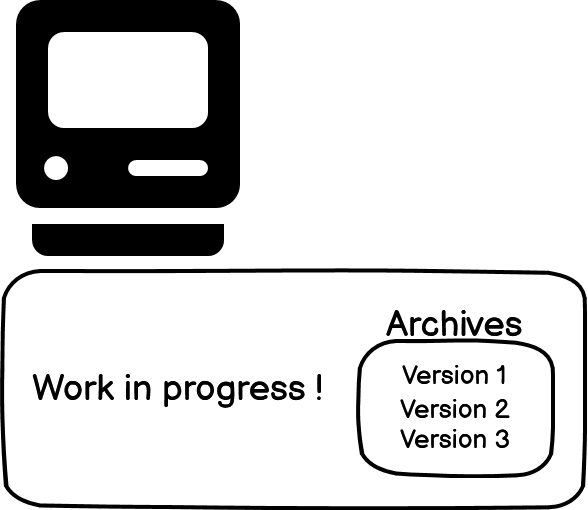
\includegraphics[scale=0.55]{images/SaveLocalNew.png}
    \end{block}
    \centering
    \footnotesize $^{*}$GNU : GNU's Not Unix
\end{frame}

\begin{frame}
    \begin{block}{Centralized VCS - Avant... un peux moins longtemps !}
     \begin{itemize}
            \item Partage plus facile
            \item Connexion réseau obligatoire (approche Client-Serveur)
        \end{itemize}
    \centering
        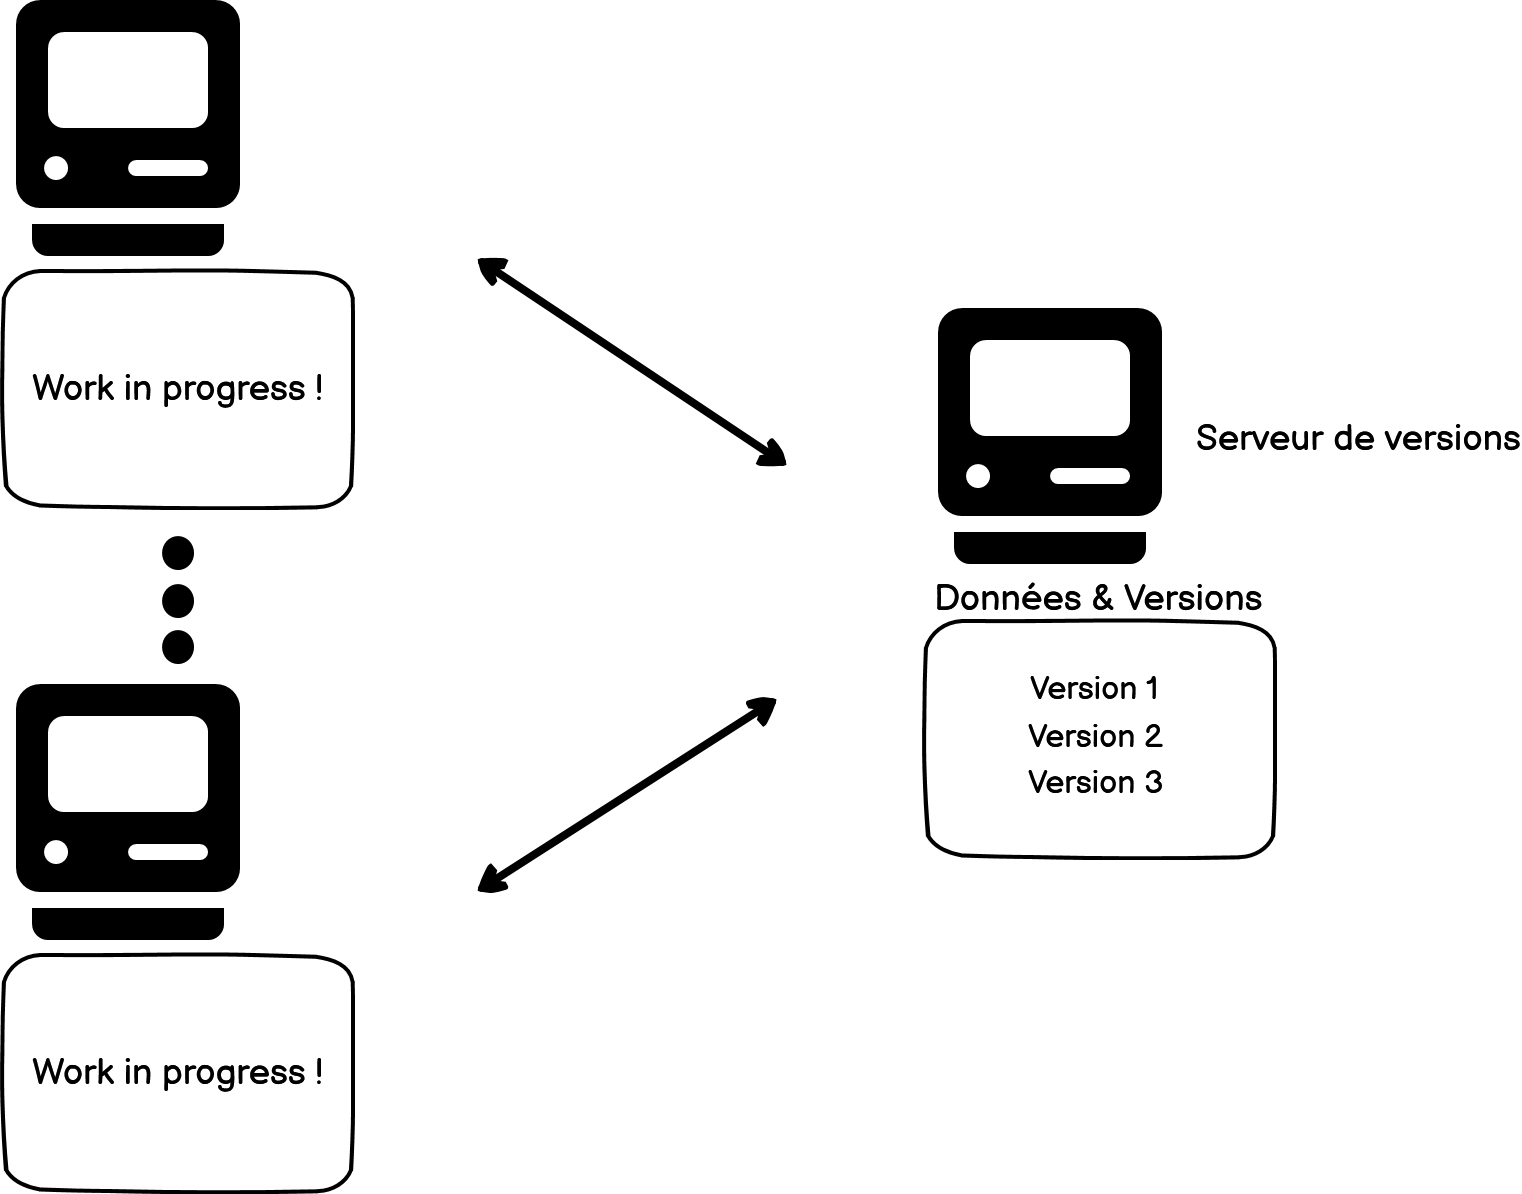
\includegraphics[scale=0.35]{images/SaveCentralNew.png}
    \end{block}
    \centering
    \footnotesize e.g. Concurrent Version System (CVS), Subversion (SVN)
\end{frame}

\begin{frame}
    \begin{block}{Distributed VCS - Maintenant, depuis un moment (début 2000) !}
     \begin{itemize}
            \item État "serveur" et réseau pas critique (approche Pair-à-Pair)
            \item On peut remonter un "serveur" à partir des autres machines
            \item Les opérations locales (la majorité) sont rapides
            \item Travail privé possible
        \end{itemize}
    \centering
        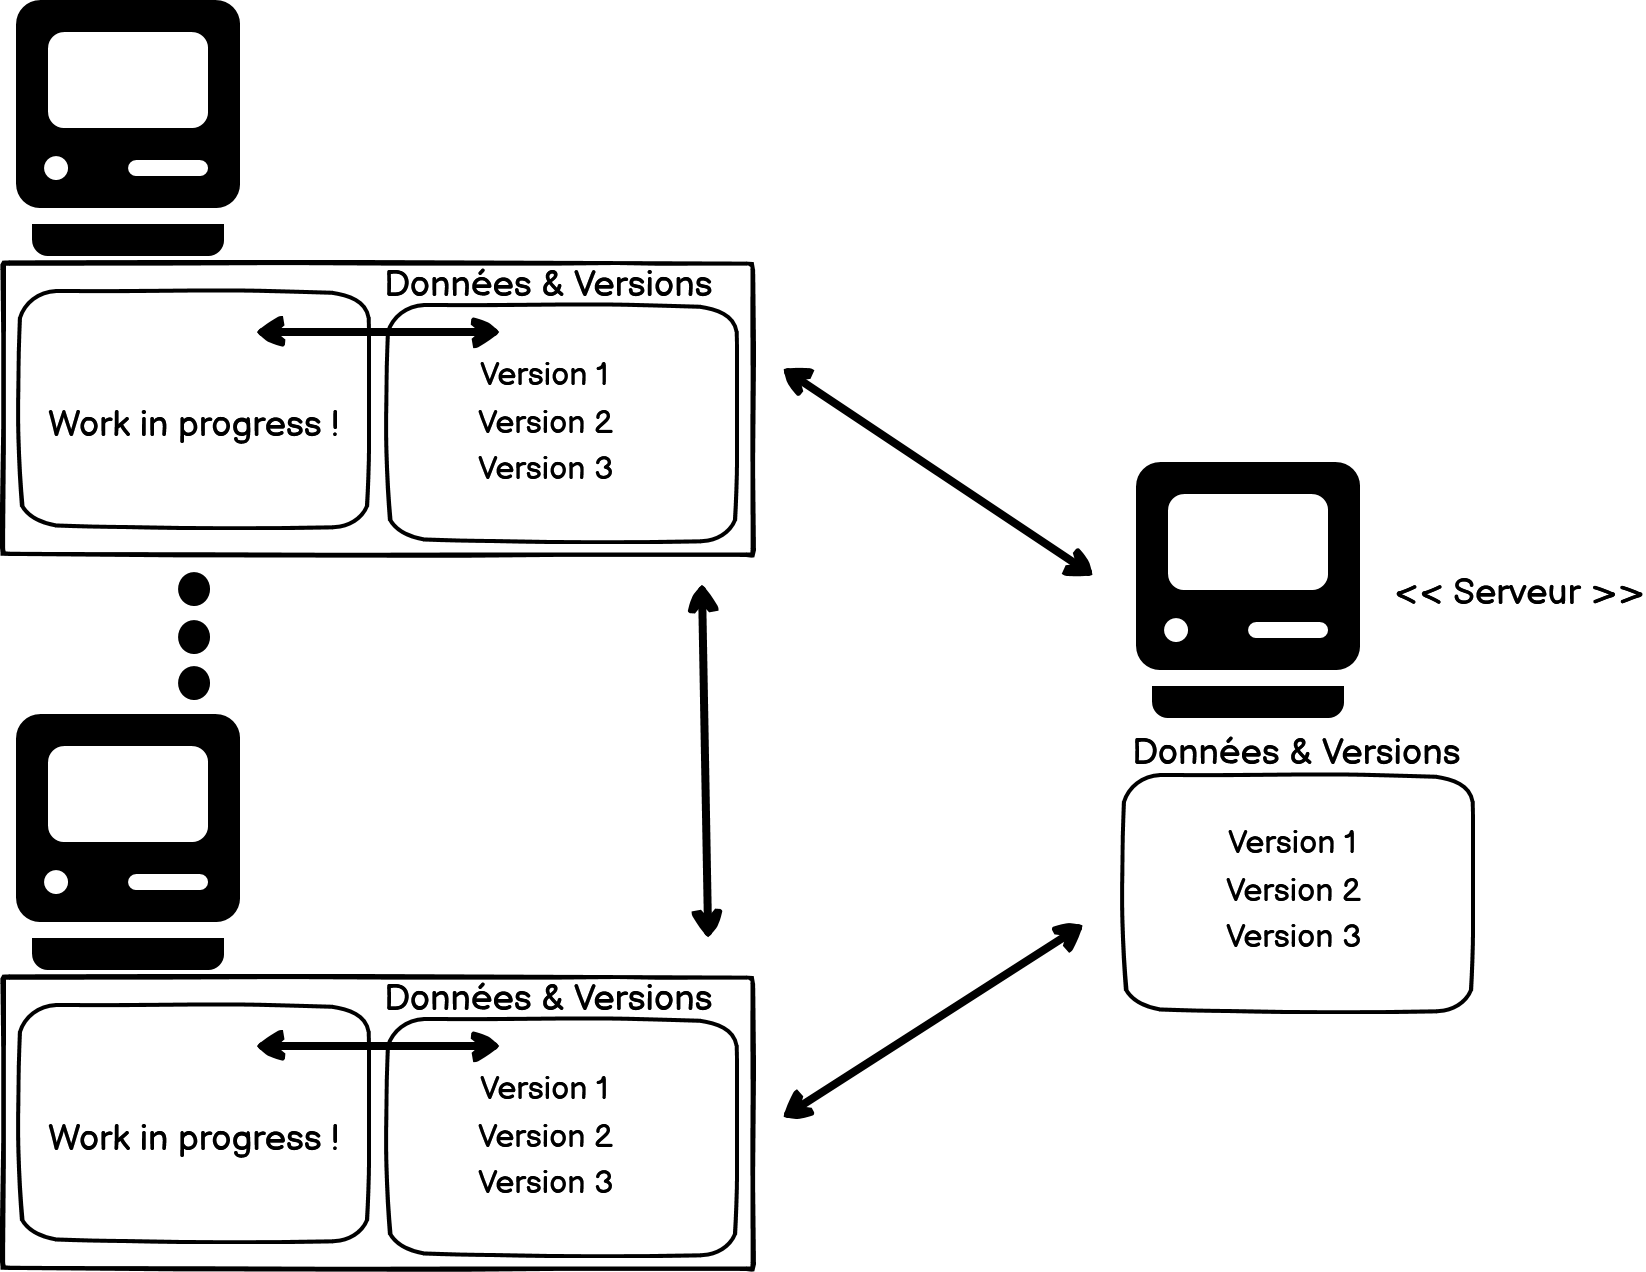
\includegraphics[scale=0.25]{images/SaveDistribNew.png}
    \end{block}
    \centering
    \footnotesize e.g. Git, Mercurial, Darcs
\end{frame}

\begin{frame}
    \begin{block}{L'origine de Git}
     \begin{itemize}
            \item Créé en 2005 par \textcolor{blue}{\textbf{\underline{\href{https://fr.wikipedia.org/wiki/Linus_Torvalds}{Linus TORVALDS}}}}
            \item Pour le noyau Linux
            \item Activement maintenu par \textcolor{blue}{\textbf{\underline{\href{https://simple.wikipedia.org/wiki/Junio_Hamano}{Junio HAMANO}}}}
            \item Popularisé par GitHub
            \item On prononce "guit" et pas "jit" !
            \item Git = Crétin (= Conna... !)                        
        \end{itemize}
    \end{block}
    \centering
\textcolor{blue}{\textbf{\underline{\href{https://fr.wikipedia.org/wiki/Git}{Git - Wikipedia}}}}
\end{frame}

\begin{frame}
    \begin{block}{Les principales caractéristiques de Git}
     \begin{itemize}
            \item Contrôle de version distribué (pair-à-pair)
            \item Gestion des branches de code (création, suppression, fusion)
            \item Opérations atomiques (Commits)
            \item Données de gestion stockée dans un répertoire .git 
        \end{itemize}
    \end{block}
\end{frame}

\subsection{Les différents modes d'utilisation}
\begin{frame}
    \begin{block}{Comment utiliser Git ?}
    \begin{itemize}
    \item En ligne de commande (Terminal \& Git Bash pour Windows)
    \item Outils graphiques intégrés à Git : "git-gui" et "gitk"
    \item Avec une IHM dans un OS (GitKraken, SourceTree) : \textcolor{blue}{\textbf{\underline{\href{https://git-scm.com/downloads/guis}{ici}}}}
    \item Intégré dans un EDI (plugin, package etc.)
    \item Sur internet : github, gitlab, bitbucket etc.
    \end{itemize}
    \centering
        
\includegraphics[scale=0.1]{images/gitkrkaen.png}
        
\includegraphics[scale=0.25]{images/sourcetree.jpg}
    \end{block}
    \centering
    \textcolor{red}{\textbf{L'apprentissage en ligne de commande est le plus efficace !}}
\end{frame}

\subsection{Le concept de branche}
\begin{frame}
\justifying
Vous avez surpris une conversation entre utilisateurs de git qui pourrait se résumer ainsi : "Il est souvent très utile, surtout quand un code est en production, d'utiliser une nouvelle branche lorsqu'on le fait évoluer !". Dans notre contexte, un code en production peut se traduire par "un code en cours d'utilisation dans le cadre d'une expérience, que l'on soit en phase d'acquisition ou de traitement des données". 
\vspace{1cm}

\centering
Vous allez suivre ce conseil !
\end{frame}

\begin{frame}

\begin{exampleblock}{Exercice \Roman{exampleBlockCounter} - Création d'une branche et étape 3 du projet}
\begin{enumerate}
    \item Créer une branche nommée "step3"
    \item Implémenter cette étape dans cette branche
\end{enumerate}
\end{exampleblock}
\justifying
\textcolor{red}{\textbf{Interruption inattendue : votre boss vous dit de changer les caractères 'r' et 's' par 'd' et 'a' pour le démarrage et l'arrêt d'un essai. Ce changement doit être opérationnel dès que possible ! (vous pourriez imaginer autre chose)}}
\begin{exampleblock}{Exercice \Roman{exampleBlockCounter} - Création d'une branche et étape 3 du projet}\stepcounter{exampleBlockCounter}
\begin{enumerate}
	\setcounter{enumi}{2}
    \item Vous retournez dans la branche main et faites les changements
    \item Vous archivez ces changements et les utilisez
    \item Vous retournez dans la branche "step3" et terminez l'étape
    \item Vous la fusionnez dans la branche principale
\end{enumerate}
\end{exampleblock}
\end{frame}

\begin{frame}

\begin{exampleblock}{Exercice \Roman{exampleBlockCounter} - Fusion de branches}
\stepcounter{exampleBlockCounter}
Pour appliquer les améliorations de l'étape 3 dans la branche principale (main) :
\begin{enumerate}
    \item Vous retournez dans la branche main
    \item Vous fusionnez la branche de l'étape 3 dans cette branche
\end{enumerate}
\end{exampleblock}
\end{frame}

\begin{frame}

\begin{alertblock}{Concepts importants à retenir}
\begin{itemize}
\item Branches
\item Commits
\item Heads (références, pointeurs)
\item Toute branche a son pointeur de même nom qui référence toujours le dernier commit de la branche
\item HEAD est le seul pointeur qui peut bouger. C'est à partir de lui que sera créé le prochain commit.
\item La fusion de branches peut être une opération délicate si de trop nombreux changements ont été effectués aux mêmes endroits dans les deux branches
\end{itemize}
\end{alertblock}

\end{frame}


\begin{frame}[containsverbatim]{Petit résumé intermédiaire}
\begin{alertblock}{Quelques Commandes : status, log, branch et switch}
    \begin{lstlisting}
$ git status             # Git status
$ git log                # Print commits
$ git log --oneline      # Print abbrev-commits
$ git branch branchName  # Create branch branchName
$ git switch branchName  # Move HEAD to branchName
$ git switch -c bName    # Create and switch to bName
    \end{lstlisting}
\end{alertblock}

\begin{alertblock}{Il existe un répertoire .git}
    \begin{itemize}
        \item Il contient la base de donnée locale du dépôt : dépôt local
        \item Il contient un fichier de configuration du dépôt
    \end{itemize}
\end{alertblock}
\end{frame}

\begin{frame}[containsverbatim]{Petit résumé intermédiaire}
\begin{alertblock}{I need help !}
    \begin{lstlisting}
$ git commit help # open html or man page on "commit"
$ git remote -h   # Quick "remote" help in console
    \end{lstlisting}
\end{alertblock}
\end{frame}

\end{document}
